% !TEX root = ../main.tex

\chapter{Introduction}
\label{ch:introduction}

Your introduction chapter here.

\section{Black-Box Optimization}
\subsection{Evolution Strategies}
Evolution Strategies (ES) ...

\subsection{Covariance Matrix Adaptation Evolution Strategy}
Covariance Matrix Adaptation Evolution Strategy (CMA-ES) ...

\section{Alternative Function Approximators}
\subsection{Polynomial}

\subsection{Fourier}

\subsection{Bézier}


\section{Previous Work}

\subsection{Benchmarks in Reinforcement Learning}
When developing a novel algorithm, we have to discover how it performs compared to existing methods.
For this evaluation, we need standard benchmark problems. OpenAI Gym \footnote{\url{gym.openai.com}} is a toolkit created for exactly this scenario. It contains a collection of benchmark problems with various levels of difficulty. However, not all benchmark problems are meaningful for the evaluation of an algorithm. If a problem is trivial to solve, the results do not reflect the quality of the model adequately. \\
In the paper \emph{Analyzing Reinforcement Learning Benchmarks with Random Weight Guessing} (\citet{oller_analyzing_2020}), the authors analyze and visualize the complexity of standard RL benchmarks based on score distribution. They tested their approach on the five Classic Control benchmarks from the OpenAI Gym interface: \verb|CartPole|, \verb|Acrobot|, \verb|Pendulum|, \verb|MountainCar|, and \verb|MountainCarContinuous|.
Given an RL environment, the authors conducted a fixed series of experiments. For these experiments, they used three NN architectures ($N_{architectures}=3$): a network without any hidden layers (0 HL), a network with a single hidden layer of 4 units (1 HL, 4 HU), and a network with two hidden layers of 4 units each (2 HL, 4 HU).
To avoid bias in the data, they did not include any learning. Instead, they chose the network weights i.i.d. from the standard normal distribution $\mathcal{N}(0,1)$ with Random Weight Guessing (RWG). With this, they initialized $10^4$ samples ($N_{samples}=10^4$) with different random weights. Each of these samples represents a controller that maps observations to actions in the environment. Therefore, neural networks denote the controllers. However, the goal of this thesis is to use an alternative function approximator representing the controller. The controllers were tested on an environment for 20 independent episodes ($N_{episodes}=20$). For each episode, they saved the score in the score tensor $S$. Algorithm~\ref{alg:environment-evaluation} illustrates the procedure with pseudocode.

\begin{algorithm}
\caption{Evaluation process taken from \citet{oller_analyzing_2020}}
\begin{algorithmic}[1]
\State Initialize environment
\State Create array $S$ of size $N_{architectures} \times N_{samples} \times N_{episodes}$
\For{$n = 1,2,...,N_{samples}$}
    \State Sample NN weights randomly from $\mathcal{N}(0,1)$
    \For{$e=1,2,...,N_{episodes}$}
      \State Reset the environment
      \State Run episode with NN
      \State Store accured episode reward in $S_{a,n,e}$
    \EndFor
\EndFor
\end{algorithmic}
\label{alg:environment-evaluation}
\end{algorithm}

After the authors obtained the scores, they calculated the mean performance over all episodes from a sample and its variance. The samples were ranked according to their mean score. They then visualized their results with three plots: a log-scale histogram of the mean scores, a scatter plot of the sample scores over their rank, a scatter plot of score variance over the mean score. I reproduced their results following the mentioned methodology. My findings for the environment \verb|CartPole| are displayed in Figure~\ref{fig:plots_reproduced}.

\begin{figure}[ht]
\centering
\begin{subfigure}{\textwidth}
  \centering
  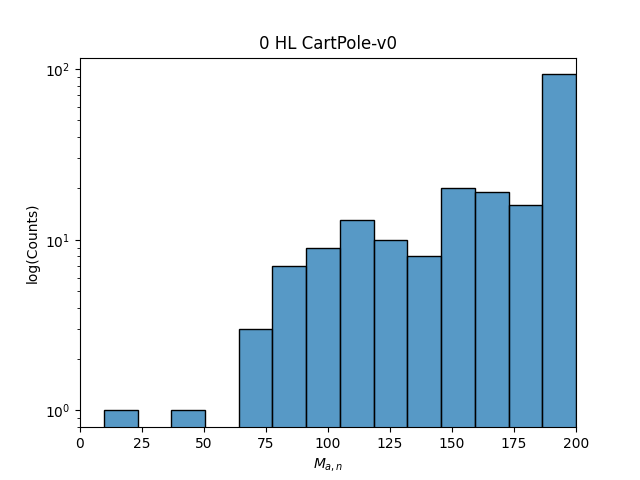
\includegraphics[width=0.329\textwidth]{histogram_zero_HL}
  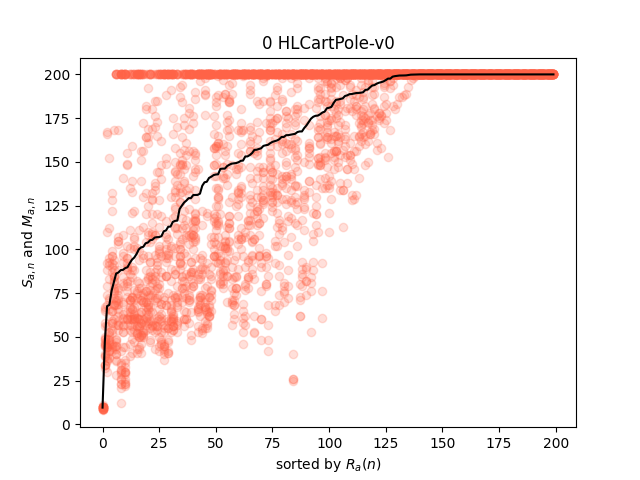
\includegraphics[width=0.329\textwidth]{scatter_score_zero_HL}
  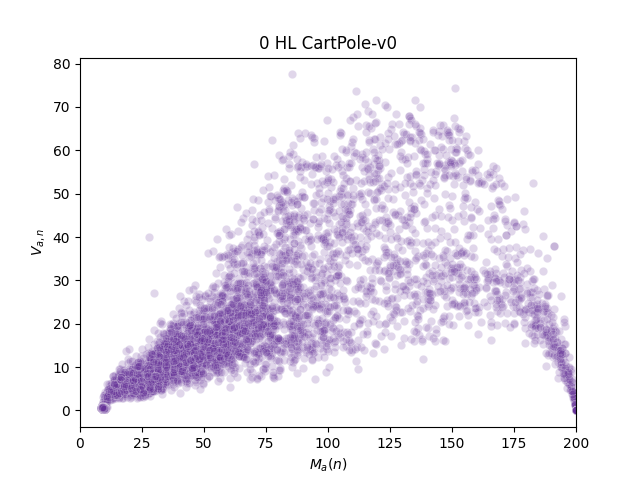
\includegraphics[width=0.329\textwidth]{scatter_variance_zero_HL}
    \caption{Results of network architecture without hidden layers}
    \label{fig:plots_reproduced_first}
\end{subfigure}
\begin{subfigure}{\textwidth}
  \centering
  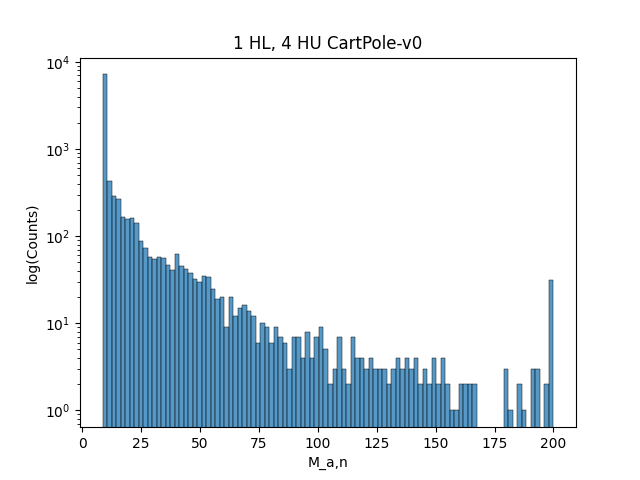
\includegraphics[width=0.329\textwidth]{histogram_one_HL}
  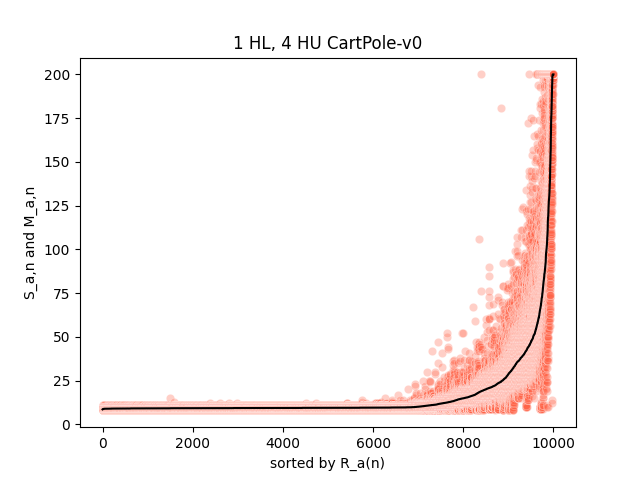
\includegraphics[width=0.329\textwidth]{scatter_score_one_HL}
  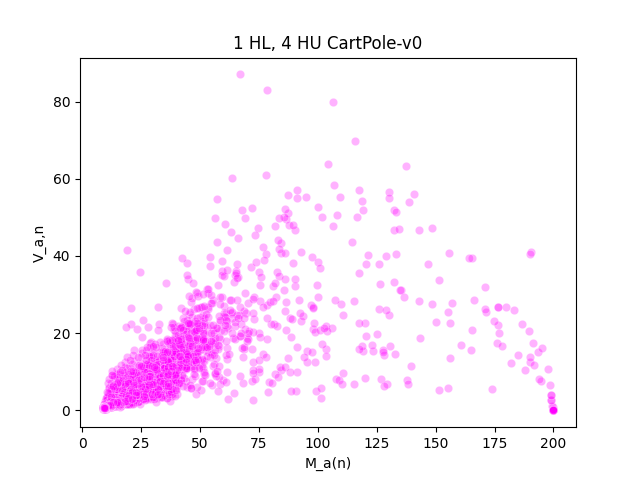
\includegraphics[width=0.329\textwidth]{scatter_variance_one_HL}
    \caption{Results of network architecture with one hidden layer}
    \label{fig:plots_reproduced_second}
\end{subfigure}
\begin{subfigure}{\textwidth}
  \centering
  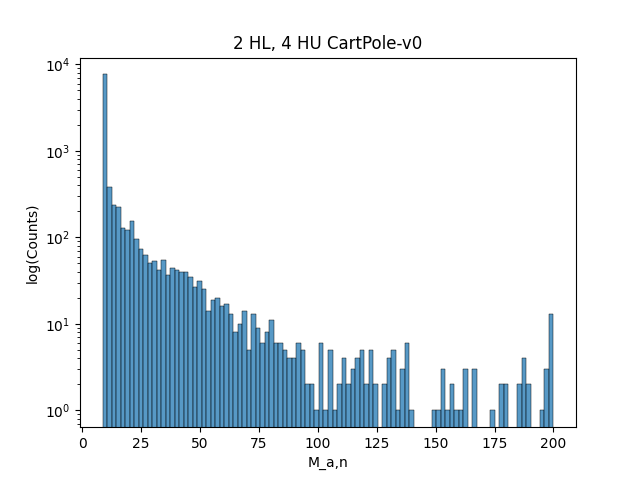
\includegraphics[width=0.329\textwidth]{histogram_two_HL}
  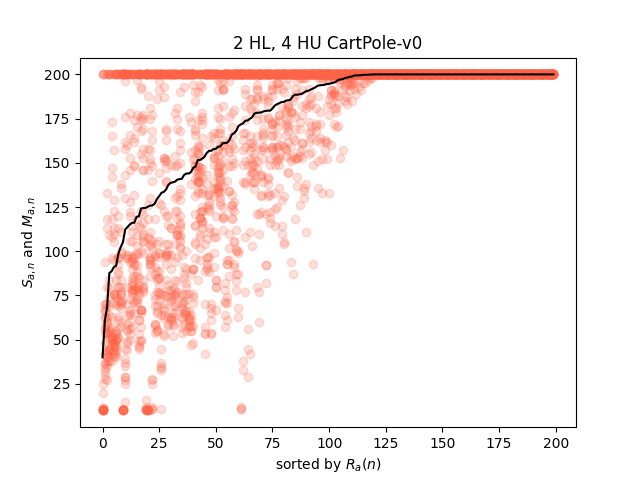
\includegraphics[width=0.329\textwidth]{scatter_score_two_HL}
  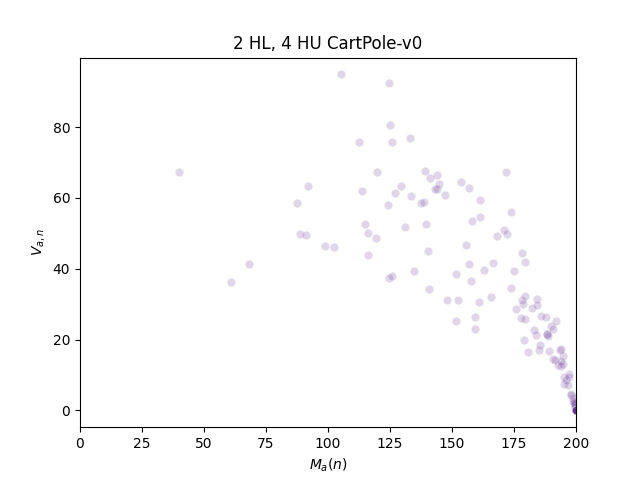
\includegraphics[width=0.329\textwidth]{scatter_variance_two_HL}
    \caption{Results of network architecture with two hidden layers}
    \label{fig:plots_reproduced_third}
\end{subfigure}
\caption[Reproduced Plots]{
  \textbf{Results.}
  Results illustrated as histogram and scatter plots.
}
\label{fig:plots_reproduced}
\end{figure}


\todo[inline]{Describe method -> results -> conclusion \\
Describe plots, maybe add plots from other environments? now not really meaningful to show all architectures (not enough difference)}
